\documentclass[11pt]{report}

% This makes easy to have the words "DVD Rental System" in bold every time
\newcommand{\DRS}{\textbf{DVD Rental System} }

% Use for including images
\usepackage{graphicx}

\begin{document}

\title{DVD Rental System Application Design}
\author{Keith Miller, Ahmed Madkour, Adrian Kosmaczewski \\ University of Liverpool \\ MSc in IT, Software Engineering}
\date{Sunday, November 5th, 2006}
\maketitle

\tableofcontents 
\listoffigures 

\chapter{Introduction}

This document presents the \DRS, which will be used by Video Fun to streamline its operations around a common, standardized set of tools. The goal of the \DRS is to reduce costs, enhance team collaboration, and integrate the whole staff of the company with a single system.

\chapter{Textual Description}

The video library Video Fun lends videos and DVDs. The \DRS will record details about the customers who use the library, the materials that are available to be lent, and record which customer currently has what materials on loan.

The details that are stored for a customer are their first and last name, their address, their phone number and their membership number.  The details that are stored for a video and a DVD are their title and serial number.  Videos can be rented for a period of one week and the rental charge is two Euros.  If a video is returned late an additional late fee is payable of one Euro per day late.  DVDs can be rented for a period of two days and the rental charge is three Euros.  If a DVD is returned late an additional late fee is payable of two Euros per day late.

The program needs to provide the functionality to allow new customers to be added to the system.  To allow new videos or DVDs to be added to the system.  To allow a video or DVD to be recorded as rented to a customer (the user would enter the customer�s membership number, the item�s serial number and the date of rental).  When an item is rented a receipt should be output to the screen that states the name of the item, the length of rental time and the cost of rental.  To record the return of a video or DVD the user would enter the serial number for the item and the date of return.  If a returned item is late an invoice should be output to the screen that states the name and address of the customer, the name of the item and the late fee.

For simplicity the program does not have to cater for deleting or editing customer details or video or DVD details.  Also for simplicity the program does not have to store or load the customer or video or DVD data from files.  (Bonus marks will be allocated to students who do implement the functionality of being able to load and save the program data to and from a file.  To implement this functionality it is easiest if there is a separate file for each type of data: customer, video and DVD.)  For testing purposes an initial set of customers and videos and DVDs can be hard coded into the system.  New customers, videos and DVDs should be able to be added to the system as it is running.

\chapter{Analysis Model}

The textual description shown in the previous chapter has been translated to the following UML diagrams:

\section{Use Case}

\begin{figure}[here]
\begin{center}
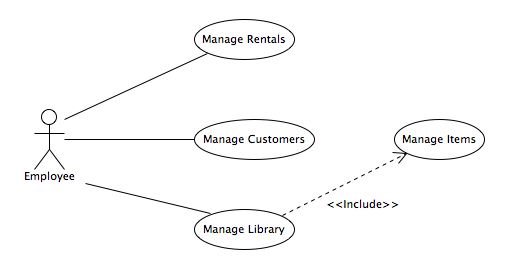
\includegraphics[width=5in]{images/usecase.png}
\caption{Use Case Diagram}
\label{useCaseDiagram}
\end{center}
\end{figure}

\section{Class Diagram}

\begin{figure}[here]
\begin{center}
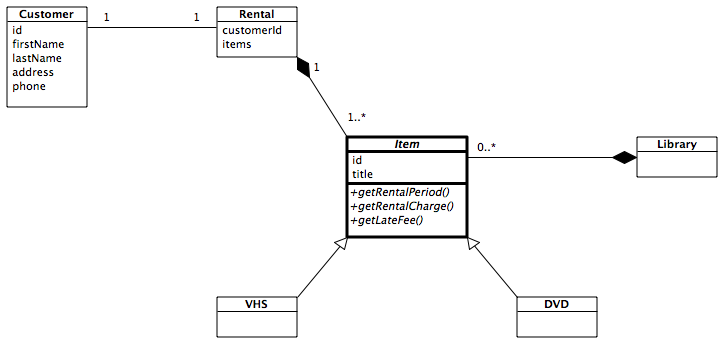
\includegraphics[width=5.5in]{images/classes.png}
\caption{Class Diagram}
\label{classDiagram}
\end{center}
\end{figure}

\section{User Interface Mock-ups}

If the \DRS was to be implemented using a graphical user interface, the following images show mock-ups of possible screens:

\begin{figure}[here]
\begin{center}
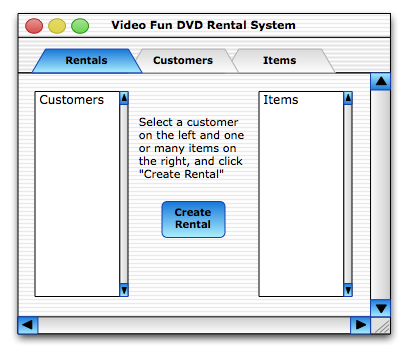
\includegraphics[width=4in]{images/ui.png}
\caption{User Interface}
\label{userInterface}
\end{center}
\end{figure}

\begin{figure}[here]
\begin{center}
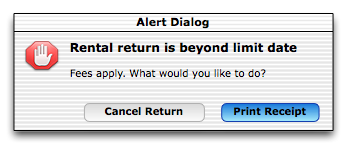
\includegraphics[width=3.5in]{images/alert.png}
\caption{Alert Dialog}
\label{alertDialog}
\end{center}
\end{figure}

\end{document}
